\begin{frame}
	\myheading{Module 8.11 : Dropout}
\end{frame}

\begin{frame}
	\vspace{4em}
	\begin{overlayarea}{\textwidth}{\textheight}
		\begin{block}{Other forms of regularization}
			\begin{itemize}
				\item $l_2$ regularization
				\item Dataset augmentation
				\item Parameter Sharing and tying
				\item Adding Noise to the inputs
				\item Adding Noise to the outputs 
				\item Early stopping
				\item Ensemble methods
				\item \textcolor<2->{red}{Dropout}
			\end{itemize}
		\end{block}
	\end{overlayarea}
\end{frame}


\begin{frame}
	\tikzstyle{input_neuron}=[circle,draw=red!50,fill=orange!10,thick,minimum size=.2mm]
	\tikzstyle{hidden_neuron}=[circle,draw=blue!50,fill=blue!10,thick,minimum size=1mm]
	\tikzstyle{output_neuron}=[circle,draw=green!50,fill=green!20,thick,minimum size=1mm]
					
	\tikzstyle{input}=[circle,draw=black!50,fill=black!20,thick,minimum size=.2mm]
	\begin{columns}
		\column{0.5\textwidth}
		\onslide<3->{\begin{minipage}[c]{.31\textwidth}
			\input{modules/Module11/tikz_images/sample_arch1.tex}
		\end{minipage}}
		\onslide<3->{\begin{minipage}[c]{0.31\textwidth}
			\input{modules/Module11/tikz_images/sample_arch2.tex}
		\end{minipage}}
		\onslide<3->{\begin{minipage}[c]{0.31\textwidth}
			\input{modules/Module11/tikz_images/sample_arch3.tex}
		\end{minipage}}								
		\onslide<4->{\begin{minipage}{0.31\textwidth}
			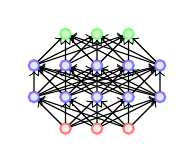
\begin{tikzpicture}[scale=.4, transform shape,cross/.style={path picture={ 
		\draw[black]
		(path picture bounding box.south east) -- (path picture bounding box.north west) (path picture bounding box.south west) -- (path picture bounding box.north east);
	}}]]
						
						
	\node [input_neuron] (in0) at (4,4) {};
	\node [input_neuron] (in1) at (5,4) {};
	\node [input_neuron] (in2) at (6,4) {} ;
						
	\node [hidden_neuron] (hi0) at (3,5)  {} ;
	\node [hidden_neuron] (hi1) at (4,5)  {};
	\node [hidden_neuron] (hi2) at (5,5)  {} ;
	\node [hidden_neuron] (hi3) at (6,5)  {} ;
	\node [hidden_neuron] (hi4) at (7,5)  {};
						
	\node [hidden_neuron] (hi01) at (3,6)  {} ;
	\node [hidden_neuron] (hi11) at (4,6)  {};
	\node [hidden_neuron] (hi21) at (5,6)  {} ;
	\node [hidden_neuron] (hi31) at (6,6)  {} ;
	\node [hidden_neuron] (hi41) at (7,6)  {};
						
	\node [output_neuron] (out0) at (4,7)  {} ;
	\node [output_neuron] (out1) at (5,7)  {} ;
	\node [output_neuron] (out2) at (6,7)  {} ;
						
						
	\draw [->] (in0) -- (hi0);
	\draw [->] (in0) -- (hi1);
	\draw [->] (in0) -- (hi2);
	\draw [->] (in0) -- (hi3);
	\draw [->] (in0) -- (hi4);
	\draw [->] (in1) -- (hi0);
	\draw [->] (in1) -- (hi1);
	\draw [->] (in1) -- (hi2);
	\draw [->] (in1) -- (hi3);
	\draw [->] (in1) -- (hi4);
	\draw [->] (in2) -- (hi0);
	\draw [->] (in2) -- (hi1);
	\draw [->] (in2) -- (hi2);
	\draw [->] (in2) -- (hi3);
	\draw [->] (in2) -- (hi4);
						
	\draw [->] (hi0) -- (hi01);
	\draw [->] (hi0) -- (hi11);
	\draw [->] (hi0) -- (hi21);
	\draw [->] (hi0) -- (hi31);
	\draw [->] (hi0) -- (hi41);
	\draw [->] (hi1) -- (hi01);
	\draw [->] (hi1) -- (hi11);
	\draw [->] (hi1) -- (hi21);
	\draw [->] (hi1) -- (hi31);
	\draw [->] (hi1) -- (hi41);
	\draw [->] (hi2) -- (hi01);
	\draw [->] (hi2) -- (hi11);
	\draw [->] (hi2) -- (hi21);
	\draw [->] (hi2) -- (hi31);
	\draw [->] (hi2) -- (hi41);
	\draw [->] (hi3) -- (hi01);
	\draw [->] (hi3) -- (hi11);
	\draw [->] (hi3) -- (hi21);
	\draw [->] (hi3) -- (hi31);
	\draw [->] (hi3) -- (hi41);
	\draw [->] (hi4) -- (hi01);
	\draw [->] (hi4) -- (hi11);
	\draw [->] (hi4) -- (hi21);
	\draw [->] (hi4) -- (hi31);
	\draw [->] (hi4) -- (hi41);
						
	\draw [->] (hi01) -- (out0);
	\draw [->] (hi01) -- (out1);
	\draw [->] (hi01) -- (out2);
	\draw [->] (hi11) -- (out0);
	\draw [->] (hi11) -- (out1);
	\draw [->] (hi11) -- (out2);
	\draw [->] (hi21) -- (out0);
	\draw [->] (hi21) -- (out1);
	\draw [->] (hi21) -- (out2);
	\draw [->] (hi31) -- (out0);
	\draw [->] (hi31) -- (out1);
	\draw [->] (hi31) -- (out2);
	\draw [->] (hi41) -- (out0);
	\draw [->] (hi41) -- (out1);
	\draw [->] (hi41) -- (out2);
\end{tikzpicture}
		\end{minipage}}
		\onslide<4->{\begin{minipage}{0.31\textwidth}
			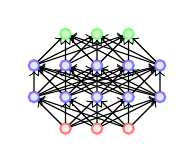
\begin{tikzpicture}[scale=.4, transform shape,cross/.style={path picture={ 
		\draw[black]
		(path picture bounding box.south east) -- (path picture bounding box.north west) (path picture bounding box.south west) -- (path picture bounding box.north east);
	}}]]
						
						
	\node [input_neuron] (in0) at (4,4) {};
	\node [input_neuron] (in1) at (5,4) {};
	\node [input_neuron] (in2) at (6,4) {} ;
						
	\node [hidden_neuron] (hi0) at (3,5)  {} ;
	\node [hidden_neuron] (hi1) at (4,5)  {};
	\node [hidden_neuron] (hi2) at (5,5)  {} ;
	\node [hidden_neuron] (hi3) at (6,5)  {} ;
	\node [hidden_neuron] (hi4) at (7,5)  {};
						
	\node [hidden_neuron] (hi01) at (3,6)  {} ;
	\node [hidden_neuron] (hi11) at (4,6)  {};
	\node [hidden_neuron] (hi21) at (5,6)  {} ;
	\node [hidden_neuron] (hi31) at (6,6)  {} ;
	\node [hidden_neuron] (hi41) at (7,6)  {};
						
	\node [output_neuron] (out0) at (4,7)  {} ;
	\node [output_neuron] (out1) at (5,7)  {} ;
	\node [output_neuron] (out2) at (6,7)  {} ;
						
						
	\draw [->] (in0) -- (hi0);
	\draw [->] (in0) -- (hi1);
	\draw [->] (in0) -- (hi2);
	\draw [->] (in0) -- (hi3);
	\draw [->] (in0) -- (hi4);
	\draw [->] (in1) -- (hi0);
	\draw [->] (in1) -- (hi1);
	\draw [->] (in1) -- (hi2);
	\draw [->] (in1) -- (hi3);
	\draw [->] (in1) -- (hi4);
	\draw [->] (in2) -- (hi0);
	\draw [->] (in2) -- (hi1);
	\draw [->] (in2) -- (hi2);
	\draw [->] (in2) -- (hi3);
	\draw [->] (in2) -- (hi4);
						
	\draw [->] (hi0) -- (hi01);
	\draw [->] (hi0) -- (hi11);
	\draw [->] (hi0) -- (hi21);
	\draw [->] (hi0) -- (hi31);
	\draw [->] (hi0) -- (hi41);
	\draw [->] (hi1) -- (hi01);
	\draw [->] (hi1) -- (hi11);
	\draw [->] (hi1) -- (hi21);
	\draw [->] (hi1) -- (hi31);
	\draw [->] (hi1) -- (hi41);
	\draw [->] (hi2) -- (hi01);
	\draw [->] (hi2) -- (hi11);
	\draw [->] (hi2) -- (hi21);
	\draw [->] (hi2) -- (hi31);
	\draw [->] (hi2) -- (hi41);
	\draw [->] (hi3) -- (hi01);
	\draw [->] (hi3) -- (hi11);
	\draw [->] (hi3) -- (hi21);
	\draw [->] (hi3) -- (hi31);
	\draw [->] (hi3) -- (hi41);
	\draw [->] (hi4) -- (hi01);
	\draw [->] (hi4) -- (hi11);
	\draw [->] (hi4) -- (hi21);
	\draw [->] (hi4) -- (hi31);
	\draw [->] (hi4) -- (hi41);
						
	\draw [->] (hi01) -- (out0);
	\draw [->] (hi01) -- (out1);
	\draw [->] (hi01) -- (out2);
	\draw [->] (hi11) -- (out0);
	\draw [->] (hi11) -- (out1);
	\draw [->] (hi11) -- (out2);
	\draw [->] (hi21) -- (out0);
	\draw [->] (hi21) -- (out1);
	\draw [->] (hi21) -- (out2);
	\draw [->] (hi31) -- (out0);
	\draw [->] (hi31) -- (out1);
	\draw [->] (hi31) -- (out2);
	\draw [->] (hi41) -- (out0);
	\draw [->] (hi41) -- (out1);
	\draw [->] (hi41) -- (out2);
\end{tikzpicture}
		\end{minipage}}
		\onslide<4->{\begin{minipage}{0.31\textwidth}
			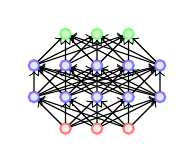
\begin{tikzpicture}[scale=.4, transform shape,cross/.style={path picture={ 
		\draw[black]
		(path picture bounding box.south east) -- (path picture bounding box.north west) (path picture bounding box.south west) -- (path picture bounding box.north east);
	}}]]
						
						
	\node [input_neuron] (in0) at (4,4) {};
	\node [input_neuron] (in1) at (5,4) {};
	\node [input_neuron] (in2) at (6,4) {} ;
						
	\node [hidden_neuron] (hi0) at (3,5)  {} ;
	\node [hidden_neuron] (hi1) at (4,5)  {};
	\node [hidden_neuron] (hi2) at (5,5)  {} ;
	\node [hidden_neuron] (hi3) at (6,5)  {} ;
	\node [hidden_neuron] (hi4) at (7,5)  {};
						
	\node [hidden_neuron] (hi01) at (3,6)  {} ;
	\node [hidden_neuron] (hi11) at (4,6)  {};
	\node [hidden_neuron] (hi21) at (5,6)  {} ;
	\node [hidden_neuron] (hi31) at (6,6)  {} ;
	\node [hidden_neuron] (hi41) at (7,6)  {};
						
	\node [output_neuron] (out0) at (4,7)  {} ;
	\node [output_neuron] (out1) at (5,7)  {} ;
	\node [output_neuron] (out2) at (6,7)  {} ;
						
						
	\draw [->] (in0) -- (hi0);
	\draw [->] (in0) -- (hi1);
	\draw [->] (in0) -- (hi2);
	\draw [->] (in0) -- (hi3);
	\draw [->] (in0) -- (hi4);
	\draw [->] (in1) -- (hi0);
	\draw [->] (in1) -- (hi1);
	\draw [->] (in1) -- (hi2);
	\draw [->] (in1) -- (hi3);
	\draw [->] (in1) -- (hi4);
	\draw [->] (in2) -- (hi0);
	\draw [->] (in2) -- (hi1);
	\draw [->] (in2) -- (hi2);
	\draw [->] (in2) -- (hi3);
	\draw [->] (in2) -- (hi4);
						
	\draw [->] (hi0) -- (hi01);
	\draw [->] (hi0) -- (hi11);
	\draw [->] (hi0) -- (hi21);
	\draw [->] (hi0) -- (hi31);
	\draw [->] (hi0) -- (hi41);
	\draw [->] (hi1) -- (hi01);
	\draw [->] (hi1) -- (hi11);
	\draw [->] (hi1) -- (hi21);
	\draw [->] (hi1) -- (hi31);
	\draw [->] (hi1) -- (hi41);
	\draw [->] (hi2) -- (hi01);
	\draw [->] (hi2) -- (hi11);
	\draw [->] (hi2) -- (hi21);
	\draw [->] (hi2) -- (hi31);
	\draw [->] (hi2) -- (hi41);
	\draw [->] (hi3) -- (hi01);
	\draw [->] (hi3) -- (hi11);
	\draw [->] (hi3) -- (hi21);
	\draw [->] (hi3) -- (hi31);
	\draw [->] (hi3) -- (hi41);
	\draw [->] (hi4) -- (hi01);
	\draw [->] (hi4) -- (hi11);
	\draw [->] (hi4) -- (hi21);
	\draw [->] (hi4) -- (hi31);
	\draw [->] (hi4) -- (hi41);
						
	\draw [->] (hi01) -- (out0);
	\draw [->] (hi01) -- (out1);
	\draw [->] (hi01) -- (out2);
	\draw [->] (hi11) -- (out0);
	\draw [->] (hi11) -- (out1);
	\draw [->] (hi11) -- (out2);
	\draw [->] (hi21) -- (out0);
	\draw [->] (hi21) -- (out1);
	\draw [->] (hi21) -- (out2);
	\draw [->] (hi31) -- (out0);
	\draw [->] (hi31) -- (out1);
	\draw [->] (hi31) -- (out2);
	\draw [->] (hi41) -- (out0);
	\draw [->] (hi41) -- (out1);
	\draw [->] (hi41) -- (out2);
\end{tikzpicture}
		\end{minipage}}
		\column{0.5\textwidth}
		\begin{overlayarea}{\textwidth}{\textheight}
			\begin{itemize}
				\justifying
				\item<1->  Typically model averaging(bagging ensemble) always helps
				\item<2-> Training several large neural networks for making an ensemble is prohibitively expensive
				\item<3->  Option 1: Train several neural networks having different architectures(obviously expensive)
				\item<4->  Option 2: Train multiple instances of the same network using different training samples (again expensive)
				\item<5->  Even if we manage to train with option 1 or option 2, combining several models at test time is infeasible in real time applications
			\end{itemize}
		\end{overlayarea}
	\end{columns}
\end{frame}
				
%  Lect 3.4   
\begin{frame}
	\tikzstyle{input_neuron}=[circle,draw=red!50,fill=orange!10,thick,minimum size=.2mm]
	\tikzstyle{hidden_neuron}=[circle,draw=blue!50,fill=blue!10,thick,minimum size=1mm]
	\tikzstyle{output_neuron}=[circle,draw=green!50,fill=green!20,thick,minimum size=1mm]
								
	\tikzstyle{input}=[circle,draw=black!50,fill=black!20,thick,minimum size=.2mm]
	\begin{columns}
						
		\column{0.5\textwidth}
		\onslide<1->{\begin{minipage}[c]{.31\textwidth}
			\input{modules/Module11/tikz_images/sample_arch1.tex}
		\end{minipage}}
		\onslide<1->{\begin{minipage}[c]{0.31\textwidth}
			\input{modules/Module11/tikz_images/sample_arch2.tex}
		\end{minipage}}
		\onslide<1->{\begin{minipage}[c]{0.31\textwidth}
			\input{modules/Module11/tikz_images/sample_arch3.tex}
		\end{minipage}}								
		\onslide<1->{\begin{minipage}{0.31\textwidth}
			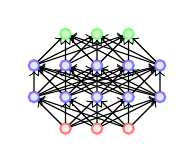
\begin{tikzpicture}[scale=.4, transform shape,cross/.style={path picture={ 
		\draw[black]
		(path picture bounding box.south east) -- (path picture bounding box.north west) (path picture bounding box.south west) -- (path picture bounding box.north east);
	}}]]
						
						
	\node [input_neuron] (in0) at (4,4) {};
	\node [input_neuron] (in1) at (5,4) {};
	\node [input_neuron] (in2) at (6,4) {} ;
						
	\node [hidden_neuron] (hi0) at (3,5)  {} ;
	\node [hidden_neuron] (hi1) at (4,5)  {};
	\node [hidden_neuron] (hi2) at (5,5)  {} ;
	\node [hidden_neuron] (hi3) at (6,5)  {} ;
	\node [hidden_neuron] (hi4) at (7,5)  {};
						
	\node [hidden_neuron] (hi01) at (3,6)  {} ;
	\node [hidden_neuron] (hi11) at (4,6)  {};
	\node [hidden_neuron] (hi21) at (5,6)  {} ;
	\node [hidden_neuron] (hi31) at (6,6)  {} ;
	\node [hidden_neuron] (hi41) at (7,6)  {};
						
	\node [output_neuron] (out0) at (4,7)  {} ;
	\node [output_neuron] (out1) at (5,7)  {} ;
	\node [output_neuron] (out2) at (6,7)  {} ;
						
						
	\draw [->] (in0) -- (hi0);
	\draw [->] (in0) -- (hi1);
	\draw [->] (in0) -- (hi2);
	\draw [->] (in0) -- (hi3);
	\draw [->] (in0) -- (hi4);
	\draw [->] (in1) -- (hi0);
	\draw [->] (in1) -- (hi1);
	\draw [->] (in1) -- (hi2);
	\draw [->] (in1) -- (hi3);
	\draw [->] (in1) -- (hi4);
	\draw [->] (in2) -- (hi0);
	\draw [->] (in2) -- (hi1);
	\draw [->] (in2) -- (hi2);
	\draw [->] (in2) -- (hi3);
	\draw [->] (in2) -- (hi4);
						
	\draw [->] (hi0) -- (hi01);
	\draw [->] (hi0) -- (hi11);
	\draw [->] (hi0) -- (hi21);
	\draw [->] (hi0) -- (hi31);
	\draw [->] (hi0) -- (hi41);
	\draw [->] (hi1) -- (hi01);
	\draw [->] (hi1) -- (hi11);
	\draw [->] (hi1) -- (hi21);
	\draw [->] (hi1) -- (hi31);
	\draw [->] (hi1) -- (hi41);
	\draw [->] (hi2) -- (hi01);
	\draw [->] (hi2) -- (hi11);
	\draw [->] (hi2) -- (hi21);
	\draw [->] (hi2) -- (hi31);
	\draw [->] (hi2) -- (hi41);
	\draw [->] (hi3) -- (hi01);
	\draw [->] (hi3) -- (hi11);
	\draw [->] (hi3) -- (hi21);
	\draw [->] (hi3) -- (hi31);
	\draw [->] (hi3) -- (hi41);
	\draw [->] (hi4) -- (hi01);
	\draw [->] (hi4) -- (hi11);
	\draw [->] (hi4) -- (hi21);
	\draw [->] (hi4) -- (hi31);
	\draw [->] (hi4) -- (hi41);
						
	\draw [->] (hi01) -- (out0);
	\draw [->] (hi01) -- (out1);
	\draw [->] (hi01) -- (out2);
	\draw [->] (hi11) -- (out0);
	\draw [->] (hi11) -- (out1);
	\draw [->] (hi11) -- (out2);
	\draw [->] (hi21) -- (out0);
	\draw [->] (hi21) -- (out1);
	\draw [->] (hi21) -- (out2);
	\draw [->] (hi31) -- (out0);
	\draw [->] (hi31) -- (out1);
	\draw [->] (hi31) -- (out2);
	\draw [->] (hi41) -- (out0);
	\draw [->] (hi41) -- (out1);
	\draw [->] (hi41) -- (out2);
\end{tikzpicture}
		\end{minipage}}
		\onslide<1->{\begin{minipage}{0.31\textwidth}
			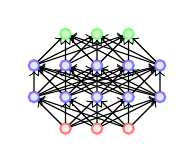
\begin{tikzpicture}[scale=.4, transform shape,cross/.style={path picture={ 
		\draw[black]
		(path picture bounding box.south east) -- (path picture bounding box.north west) (path picture bounding box.south west) -- (path picture bounding box.north east);
	}}]]
						
						
	\node [input_neuron] (in0) at (4,4) {};
	\node [input_neuron] (in1) at (5,4) {};
	\node [input_neuron] (in2) at (6,4) {} ;
						
	\node [hidden_neuron] (hi0) at (3,5)  {} ;
	\node [hidden_neuron] (hi1) at (4,5)  {};
	\node [hidden_neuron] (hi2) at (5,5)  {} ;
	\node [hidden_neuron] (hi3) at (6,5)  {} ;
	\node [hidden_neuron] (hi4) at (7,5)  {};
						
	\node [hidden_neuron] (hi01) at (3,6)  {} ;
	\node [hidden_neuron] (hi11) at (4,6)  {};
	\node [hidden_neuron] (hi21) at (5,6)  {} ;
	\node [hidden_neuron] (hi31) at (6,6)  {} ;
	\node [hidden_neuron] (hi41) at (7,6)  {};
						
	\node [output_neuron] (out0) at (4,7)  {} ;
	\node [output_neuron] (out1) at (5,7)  {} ;
	\node [output_neuron] (out2) at (6,7)  {} ;
						
						
	\draw [->] (in0) -- (hi0);
	\draw [->] (in0) -- (hi1);
	\draw [->] (in0) -- (hi2);
	\draw [->] (in0) -- (hi3);
	\draw [->] (in0) -- (hi4);
	\draw [->] (in1) -- (hi0);
	\draw [->] (in1) -- (hi1);
	\draw [->] (in1) -- (hi2);
	\draw [->] (in1) -- (hi3);
	\draw [->] (in1) -- (hi4);
	\draw [->] (in2) -- (hi0);
	\draw [->] (in2) -- (hi1);
	\draw [->] (in2) -- (hi2);
	\draw [->] (in2) -- (hi3);
	\draw [->] (in2) -- (hi4);
						
	\draw [->] (hi0) -- (hi01);
	\draw [->] (hi0) -- (hi11);
	\draw [->] (hi0) -- (hi21);
	\draw [->] (hi0) -- (hi31);
	\draw [->] (hi0) -- (hi41);
	\draw [->] (hi1) -- (hi01);
	\draw [->] (hi1) -- (hi11);
	\draw [->] (hi1) -- (hi21);
	\draw [->] (hi1) -- (hi31);
	\draw [->] (hi1) -- (hi41);
	\draw [->] (hi2) -- (hi01);
	\draw [->] (hi2) -- (hi11);
	\draw [->] (hi2) -- (hi21);
	\draw [->] (hi2) -- (hi31);
	\draw [->] (hi2) -- (hi41);
	\draw [->] (hi3) -- (hi01);
	\draw [->] (hi3) -- (hi11);
	\draw [->] (hi3) -- (hi21);
	\draw [->] (hi3) -- (hi31);
	\draw [->] (hi3) -- (hi41);
	\draw [->] (hi4) -- (hi01);
	\draw [->] (hi4) -- (hi11);
	\draw [->] (hi4) -- (hi21);
	\draw [->] (hi4) -- (hi31);
	\draw [->] (hi4) -- (hi41);
						
	\draw [->] (hi01) -- (out0);
	\draw [->] (hi01) -- (out1);
	\draw [->] (hi01) -- (out2);
	\draw [->] (hi11) -- (out0);
	\draw [->] (hi11) -- (out1);
	\draw [->] (hi11) -- (out2);
	\draw [->] (hi21) -- (out0);
	\draw [->] (hi21) -- (out1);
	\draw [->] (hi21) -- (out2);
	\draw [->] (hi31) -- (out0);
	\draw [->] (hi31) -- (out1);
	\draw [->] (hi31) -- (out2);
	\draw [->] (hi41) -- (out0);
	\draw [->] (hi41) -- (out1);
	\draw [->] (hi41) -- (out2);
\end{tikzpicture}
		\end{minipage}}
		\onslide<1->{\begin{minipage}{0.31\textwidth}
			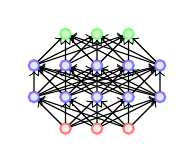
\begin{tikzpicture}[scale=.4, transform shape,cross/.style={path picture={ 
		\draw[black]
		(path picture bounding box.south east) -- (path picture bounding box.north west) (path picture bounding box.south west) -- (path picture bounding box.north east);
	}}]]
						
						
	\node [input_neuron] (in0) at (4,4) {};
	\node [input_neuron] (in1) at (5,4) {};
	\node [input_neuron] (in2) at (6,4) {} ;
						
	\node [hidden_neuron] (hi0) at (3,5)  {} ;
	\node [hidden_neuron] (hi1) at (4,5)  {};
	\node [hidden_neuron] (hi2) at (5,5)  {} ;
	\node [hidden_neuron] (hi3) at (6,5)  {} ;
	\node [hidden_neuron] (hi4) at (7,5)  {};
						
	\node [hidden_neuron] (hi01) at (3,6)  {} ;
	\node [hidden_neuron] (hi11) at (4,6)  {};
	\node [hidden_neuron] (hi21) at (5,6)  {} ;
	\node [hidden_neuron] (hi31) at (6,6)  {} ;
	\node [hidden_neuron] (hi41) at (7,6)  {};
						
	\node [output_neuron] (out0) at (4,7)  {} ;
	\node [output_neuron] (out1) at (5,7)  {} ;
	\node [output_neuron] (out2) at (6,7)  {} ;
						
						
	\draw [->] (in0) -- (hi0);
	\draw [->] (in0) -- (hi1);
	\draw [->] (in0) -- (hi2);
	\draw [->] (in0) -- (hi3);
	\draw [->] (in0) -- (hi4);
	\draw [->] (in1) -- (hi0);
	\draw [->] (in1) -- (hi1);
	\draw [->] (in1) -- (hi2);
	\draw [->] (in1) -- (hi3);
	\draw [->] (in1) -- (hi4);
	\draw [->] (in2) -- (hi0);
	\draw [->] (in2) -- (hi1);
	\draw [->] (in2) -- (hi2);
	\draw [->] (in2) -- (hi3);
	\draw [->] (in2) -- (hi4);
						
	\draw [->] (hi0) -- (hi01);
	\draw [->] (hi0) -- (hi11);
	\draw [->] (hi0) -- (hi21);
	\draw [->] (hi0) -- (hi31);
	\draw [->] (hi0) -- (hi41);
	\draw [->] (hi1) -- (hi01);
	\draw [->] (hi1) -- (hi11);
	\draw [->] (hi1) -- (hi21);
	\draw [->] (hi1) -- (hi31);
	\draw [->] (hi1) -- (hi41);
	\draw [->] (hi2) -- (hi01);
	\draw [->] (hi2) -- (hi11);
	\draw [->] (hi2) -- (hi21);
	\draw [->] (hi2) -- (hi31);
	\draw [->] (hi2) -- (hi41);
	\draw [->] (hi3) -- (hi01);
	\draw [->] (hi3) -- (hi11);
	\draw [->] (hi3) -- (hi21);
	\draw [->] (hi3) -- (hi31);
	\draw [->] (hi3) -- (hi41);
	\draw [->] (hi4) -- (hi01);
	\draw [->] (hi4) -- (hi11);
	\draw [->] (hi4) -- (hi21);
	\draw [->] (hi4) -- (hi31);
	\draw [->] (hi4) -- (hi41);
						
	\draw [->] (hi01) -- (out0);
	\draw [->] (hi01) -- (out1);
	\draw [->] (hi01) -- (out2);
	\draw [->] (hi11) -- (out0);
	\draw [->] (hi11) -- (out1);
	\draw [->] (hi11) -- (out2);
	\draw [->] (hi21) -- (out0);
	\draw [->] (hi21) -- (out1);
	\draw [->] (hi21) -- (out2);
	\draw [->] (hi31) -- (out0);
	\draw [->] (hi31) -- (out1);
	\draw [->] (hi31) -- (out2);
	\draw [->] (hi41) -- (out0);
	\draw [->] (hi41) -- (out1);
	\draw [->] (hi41) -- (out2);
\end{tikzpicture}
		\end{minipage}}									
		\column{0.5\textwidth}
		\begin{overlayarea}{\textwidth}{\textheight}
			\begin{itemize}
				\justifying
				\item Dropout is a technique which addresses both these issues.
				\item<2-> Effectively it allows training several neural networks without any significant computational overhead.
				\item<3-> Also gives an efficient approximate way of combining exponentially many different neural networks.
			\end{itemize}
		\end{overlayarea}
	\end{columns}
\end{frame}

\begin{frame}
	\tikzstyle{input_neuron}=[circle,draw=red!50,fill=orange!10,thick,minimum size=.2mm]
\tikzstyle{hidden_neuron}=[circle,draw=blue!50,fill=blue!10,thick,minimum size=1mm]
\tikzstyle{output_neuron}=[circle,draw=green!50,fill=green!20,thick,minimum size=1mm]			
\tikzstyle{input}=[circle,draw=black!50,fill=black!20,thick,minimum size=.2mm]
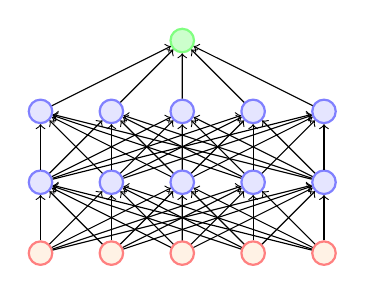
\begin{tikzpicture}[scale=.9, transform shape]
	%\tikzstyle{every node} = [draw,shape=circle]
	\node[input_neuron] (a0) at (0, 0) {};
	\node[input_neuron] (a1) at (1, 0) {};
	\node[input_neuron] (a2) at (2, 0) {};
	\node[input_neuron] (a3) at (3, 0) {};
	\node[input_neuron] (a4) at (4, 0) {};
	\node[hidden_neuron] (b0) at (0, 1) {};
	\node[hidden_neuron] (b1) at (1, 1) {};
	\node[hidden_neuron] (b2) at (2, 1) {};
	\node[hidden_neuron] (b3) at (3, 1) {};
	\node[hidden_neuron] (b4) at (4, 1) {};
	\node[hidden_neuron] (c0) at (0, 2) {};
	\node[hidden_neuron] (c1) at (1, 2) {};
	\node[hidden_neuron] (c2) at (2, 2) {};
	\node[hidden_neuron] (c3) at (3, 2) {};
	\node[hidden_neuron] (c4) at (4, 2) {};
	\node[output_neuron] (d2) at (2, 3) {};
	\foreach \from in {a0,a1,a2,a3,a4}
	\foreach \to in {b0,b1,b2,b3,b4}
	\draw [->] (\from) -- (\to);
	\foreach \from in {b0,b1,b2,b3,b4}
	\foreach \to in {c0,c1,c2,c3,c4}
	\draw [->] (\from) -- (\to);
	\foreach \from in {c0,c1,c2,c3,c4}
	\draw [->] (\from) -- (d2);
\end{tikzpicture}
	\hspace{2cm}
	\onslide<2->{
		\input{modules/Module11/tikz_images/dropout_network2.tex}
	}
	\begin{itemize}
		\item Dropout refers to dropping out units
		\item<2-> Temporarily remove a node and all its incoming/outgoing connections resulting in a thinned network
		\item<3-> Each node is retained with a fixed probability (typically $p=0.5$) for hidden nodes and $p=0.8$ for visible nodes
	\end{itemize}				
\end{frame}
			
\begin{frame}			
	\tikzstyle{input_neuron}=[circle,draw=red!50,fill=orange!10,thick,minimum size=.2mm]
\tikzstyle{hidden_neuron}=[circle,draw=blue!50,fill=blue!10,thick,minimum size=1mm]
\tikzstyle{output_neuron}=[circle,draw=green!50,fill=green!20,thick,minimum size=1mm]			
\tikzstyle{input}=[circle,draw=black!50,fill=black!20,thick,minimum size=.2mm]
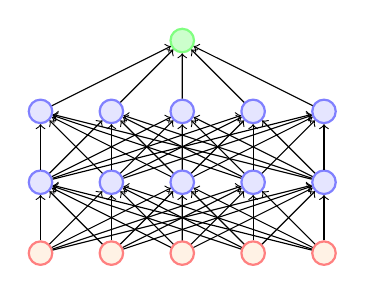
\begin{tikzpicture}[scale=.9, transform shape]
	%\tikzstyle{every node} = [draw,shape=circle]
	\node[input_neuron] (a0) at (0, 0) {};
	\node[input_neuron] (a1) at (1, 0) {};
	\node[input_neuron] (a2) at (2, 0) {};
	\node[input_neuron] (a3) at (3, 0) {};
	\node[input_neuron] (a4) at (4, 0) {};
	\node[hidden_neuron] (b0) at (0, 1) {};
	\node[hidden_neuron] (b1) at (1, 1) {};
	\node[hidden_neuron] (b2) at (2, 1) {};
	\node[hidden_neuron] (b3) at (3, 1) {};
	\node[hidden_neuron] (b4) at (4, 1) {};
	\node[hidden_neuron] (c0) at (0, 2) {};
	\node[hidden_neuron] (c1) at (1, 2) {};
	\node[hidden_neuron] (c2) at (2, 2) {};
	\node[hidden_neuron] (c3) at (3, 2) {};
	\node[hidden_neuron] (c4) at (4, 2) {};
	\node[output_neuron] (d2) at (2, 3) {};
	\foreach \from in {a0,a1,a2,a3,a4}
	\foreach \to in {b0,b1,b2,b3,b4}
	\draw [->] (\from) -- (\to);
	\foreach \from in {b0,b1,b2,b3,b4}
	\foreach \to in {c0,c1,c2,c3,c4}
	\draw [->] (\from) -- (\to);
	\foreach \from in {c0,c1,c2,c3,c4}
	\draw [->] (\from) -- (d2);
\end{tikzpicture}
	\hspace{2cm}
	\input{modules/Module11/tikz_images/dropout_network2.tex}
	\begin{itemize}
		\justifying
		\item<2-> Suppose a neural network has $n$ nodes
		\item<3-> Using the dropout idea, each node can be retained or dropped
		\item<4-> For example, in the above case we drop $5$ nodes to get a thinned network
		\item<5-> Given a total of $n$ nodes, what are the total number of thinned networks that can be formed?\onslide<6-> { $2^n$}
		\item<7-> Of course, this is prohibitively large and we cannot possibly train so many networks
		\item<8-> \textbf{Trick:} (1) Share the weights across all the networks \onslide<9-> {\\(2) Sample a different network for each training instance}
		\item<10-> Let us see how?	
	\end{itemize}
							
\end{frame}

\begin{frame}			
	\tikzstyle{input_neuron}=[circle,draw=red!50,fill=orange!10,thick,minimum size=.2mm]
\tikzstyle{hidden_neuron}=[circle,draw=blue!50,fill=blue!10,thick,minimum size=1mm]
\tikzstyle{output_neuron}=[circle,draw=green!50,fill=green!20,thick,minimum size=1mm]			
\tikzstyle{input}=[circle,draw=black!50,fill=black!20,thick,minimum size=.2mm]
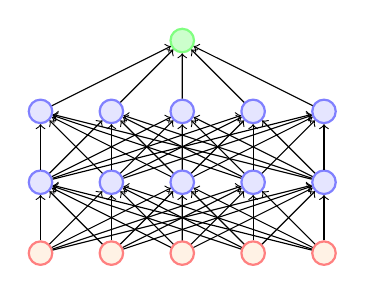
\begin{tikzpicture}[scale=.9, transform shape]
	%\tikzstyle{every node} = [draw,shape=circle]
	\node[input_neuron] (a0) at (0, 0) {};
	\node[input_neuron] (a1) at (1, 0) {};
	\node[input_neuron] (a2) at (2, 0) {};
	\node[input_neuron] (a3) at (3, 0) {};
	\node[input_neuron] (a4) at (4, 0) {};
	\node[hidden_neuron] (b0) at (0, 1) {};
	\node[hidden_neuron] (b1) at (1, 1) {};
	\node[hidden_neuron] (b2) at (2, 1) {};
	\node[hidden_neuron] (b3) at (3, 1) {};
	\node[hidden_neuron] (b4) at (4, 1) {};
	\node[hidden_neuron] (c0) at (0, 2) {};
	\node[hidden_neuron] (c1) at (1, 2) {};
	\node[hidden_neuron] (c2) at (2, 2) {};
	\node[hidden_neuron] (c3) at (3, 2) {};
	\node[hidden_neuron] (c4) at (4, 2) {};
	\node[output_neuron] (d2) at (2, 3) {};
	\foreach \from in {a0,a1,a2,a3,a4}
	\foreach \to in {b0,b1,b2,b3,b4}
	\draw [->] (\from) -- (\to);
	\foreach \from in {b0,b1,b2,b3,b4}
	\foreach \to in {c0,c1,c2,c3,c4}
	\draw [->] (\from) -- (\to);
	\foreach \from in {c0,c1,c2,c3,c4}
	\draw [->] (\from) -- (d2);
\end{tikzpicture}
	\hspace{2cm}
	\onslide<3-> {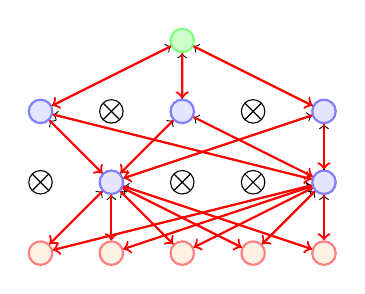
\begin{tikzpicture}[scale=.9, transform shape,cross/.style={path picture={ 
		\draw[black]
		(path picture bounding box.south east) -- (path picture bounding box.north west) (path picture bounding box.south west) -- (path picture bounding box.north east);
	}}]]
	\tikzstyle{mynode} = [draw,shape=circle]
	\tikzstyle{mycross} = [draw,shape=circle,cross]
	\node[input_neuron,mynode] (a0) at (0, 0) {};
	\node[input_neuron,mynode] (a1) at (1, 0) {};
	\node[input_neuron,mynode] (a2) at (2, 0) {};
	\node[input_neuron,mynode] (a3) at (3, 0) {};
	\node[input_neuron,mynode] (a4) at (4, 0) {};
	\node[mycross] (b0) at (0, 1) {};
	\node[hidden_neuron,mynode] (b1) at (1, 1) {};
	\node[mycross] (b2) at (2, 1) {};
	\node[mycross] (b3) at (3, 1) {};
	\node[hidden_neuron,mynode] (b4) at (4, 1) {};
	\node[hidden_neuron,mynode] (c0) at (0, 2) {};
	\node[mycross] (c1) at (1, 2) {};
	\node[hidden_neuron,mynode] (c2) at (2, 2) {};
	\node[mycross] (c3) at (3, 2) {};
	\node[hidden_neuron,mynode] (c4) at (4, 2) {};
	\node[output_neuron,mynode] (d2) at (2, 3) {};
	\foreach \from in {a0,a1,a2,a3,a4}
		\foreach \to in {b1,b4}
			\draw [->] (\from) -- (\to);
	\foreach \from in {b1,b4}
		\foreach \to in {c0,c2,c4}
			\draw [->] (\from) -- (\to);
	\foreach \from in {c0,c2,c4}
		\draw [->] (\from) -- (d2);
	\foreach \from in {c0,c2,c4}
		\draw<8-> [thick,red,->] (d2) -- (\from);
	\foreach \from in {b1,b4}
		\foreach \to in {c0,c2,c4}
			\draw<9-> [thick,red,->] (\to) -- (\from);
	\foreach \from in {a0,a1,a2,a3,a4}
		\foreach \to in {b1,b4}
			\draw<10-> [thick,red,->] (\to) -- (\from);
\end{tikzpicture}
}
	\begin{itemize}
		\justifying
		\item<2-> We initialize all the parameters (weights) of the network and start training
		\item<3-> For the first training instance (or mini-batch), we apply dropout resulting in the thinned network
		\item<4-> We compute the loss and backpropagate
		\item<5-> Which parameters will we update? \onslide<6-> { Only those which are active}
	\end{itemize}
							
\end{frame}

\begin{frame}			
	\tikzstyle{input_neuron}=[circle,draw=red!50,fill=orange!10,thick,minimum size=.2mm]
\tikzstyle{hidden_neuron}=[circle,draw=blue!50,fill=blue!10,thick,minimum size=1mm]
\tikzstyle{output_neuron}=[circle,draw=green!50,fill=green!20,thick,minimum size=1mm]			
\tikzstyle{input}=[circle,draw=black!50,fill=black!20,thick,minimum size=.2mm]
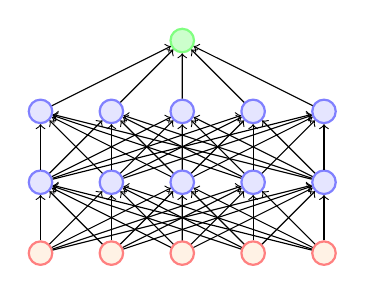
\begin{tikzpicture}[scale=.9, transform shape]
	%\tikzstyle{every node} = [draw,shape=circle]
	\node[input_neuron] (a0) at (0, 0) {};
	\node[input_neuron] (a1) at (1, 0) {};
	\node[input_neuron] (a2) at (2, 0) {};
	\node[input_neuron] (a3) at (3, 0) {};
	\node[input_neuron] (a4) at (4, 0) {};
	\node[hidden_neuron] (b0) at (0, 1) {};
	\node[hidden_neuron] (b1) at (1, 1) {};
	\node[hidden_neuron] (b2) at (2, 1) {};
	\node[hidden_neuron] (b3) at (3, 1) {};
	\node[hidden_neuron] (b4) at (4, 1) {};
	\node[hidden_neuron] (c0) at (0, 2) {};
	\node[hidden_neuron] (c1) at (1, 2) {};
	\node[hidden_neuron] (c2) at (2, 2) {};
	\node[hidden_neuron] (c3) at (3, 2) {};
	\node[hidden_neuron] (c4) at (4, 2) {};
	\node[output_neuron] (d2) at (2, 3) {};
	\foreach \from in {a0,a1,a2,a3,a4}
	\foreach \to in {b0,b1,b2,b3,b4}
	\draw [->] (\from) -- (\to);
	\foreach \from in {b0,b1,b2,b3,b4}
	\foreach \to in {c0,c1,c2,c3,c4}
	\draw [->] (\from) -- (\to);
	\foreach \from in {c0,c1,c2,c3,c4}
	\draw [->] (\from) -- (d2);
\end{tikzpicture}
	\input{modules/Module11/tikz_images/f_backprop_dropout_network2.tex}
	\only<1->{\tikzstyle{input_neuron}=[circle,draw=red!50,fill=orange!10,thick,minimum size=.2mm]
\tikzstyle{hidden_neuron}=[circle,draw=blue!50,fill=blue!10,thick,minimum size=1mm]
\tikzstyle{output_neuron}=[circle,draw=green!50,fill=green!20,thick,minimum size=1mm]
\tikzstyle{input}=[circle,draw=black!50,fill=black!20,thick,minimum size=.2mm]
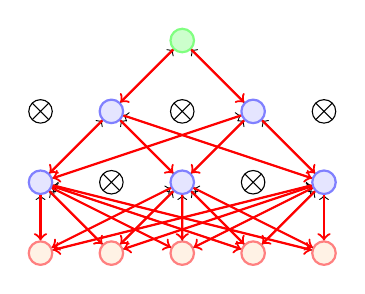
\begin{tikzpicture}[scale=.9, transform shape,cross/.style={path picture={ 
		\draw[black]
		(path picture bounding box.south east) -- (path picture bounding box.north west) (path picture bounding box.south west) -- (path picture bounding box.north east);
	}}]]
	\tikzstyle{mynode} = [draw,shape=circle]
	\tikzstyle{mycross} = [draw,shape=circle,cross]
	\node[input_neuron,mynode] (a0) at (0, 0) {};
	\node[input_neuron,mynode] (a1) at (1, 0) {};
	\node[input_neuron,mynode] (a2) at (2, 0) {};
	\node[input_neuron,mynode] (a3) at (3, 0) {};
	\node[input_neuron,mynode] (a4) at (4, 0) {};
	\node[hidden_neuron,mynode] (b0) at (0, 1) {};
	\node[mycross] (b1) at (1, 1) {};
	\node[hidden_neuron,mynode] (b2) at (2, 1) {};
	\node[mycross] (b3) at (3, 1) {};
	\node[hidden_neuron,mynode] (b4) at (4, 1) {};
	\node[mycross] (c0) at (0, 2) {};
	\node[hidden_neuron,mynode] (c1) at (1, 2) {};
	\node[mycross] (c2) at (2, 2) {};
	\node[hidden_neuron,mynode] (c3) at (3, 2) {};
	\node[mycross] (c4) at (4, 2) {};
	\node[output_neuron,mynode] (d2) at (2, 3) {};
	\foreach \from in {a0,a1,a2,a3,a4}
		\foreach \to in {b0,b2,b4}
			\draw [->] (\from) -- (\to);
	\foreach \from in {b0,b2,b4}
		\foreach \to in {c1,c3}
			\draw [->] (\from) -- (\to);
	\foreach \from in {c1,c3}
		\draw [->] (\from) -- (d2);
	%
	\foreach \from in {c1,c3}
		\draw<3-> [thick,red,->] (d2) -- (\from);
	\foreach \from in {b0,b2,b4}
		\foreach \to in {c1,c3}
			\draw<3-> [thick,red,->] (\to) -- (\from);
	\foreach \from in {a0,a1,a2,a3,a4}
		\foreach \to in {b0,b2,b4}
			\draw<3-> [thick,red,->] (\to) -- (\from);

		
		%%%
				
\end{tikzpicture}

}	
	
	%\only<3->{\input{modules/Module11/tikz_images/f_backprop_dropout2_network2.tex}}
	
\begin{itemize}
		\justifying
		\item<1-> For the second training instance (or mini-batch), we again apply dropout resulting in a different thinned network
		\item<2-> We again compute the loss and backpropagate to the active weights
		\item<4-> If the weight was active for both the training instances then it would have received two updates by now
		\item<5-> If the weight was active for only one of the training instances then it would have received only one updates by now
		\item<6-> Each thinned network gets trained rarely (or even never) but the parameter sharing ensures that no model has untrained or poorly trained parameters
	\end{itemize}
							
\end{frame}


\begin{frame}
	\tikzstyle{input_neuron}=[circle,draw=red!50,fill=orange!10,thick,minimum size=.2mm]
\tikzstyle{hidden_neuron}=[circle,draw=blue!50,fill=blue!10,thick,minimum size=1mm]
\tikzstyle{output_neuron}=[circle,draw=green!50,fill=green!20,thick,minimum size=1mm]			
\tikzstyle{input}=[circle,draw=black!50,fill=black!20,thick,minimum size=.2mm]
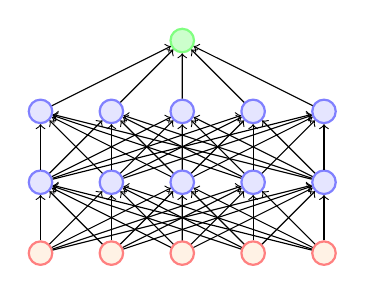
\begin{tikzpicture}[scale=.9, transform shape]
	%\tikzstyle{every node} = [draw,shape=circle]
	\node[input_neuron] (a0) at (0, 0) {};
	\node[input_neuron] (a1) at (1, 0) {};
	\node[input_neuron] (a2) at (2, 0) {};
	\node[input_neuron] (a3) at (3, 0) {};
	\node[input_neuron] (a4) at (4, 0) {};
	\node[hidden_neuron] (b0) at (0, 1) {};
	\node[hidden_neuron] (b1) at (1, 1) {};
	\node[hidden_neuron] (b2) at (2, 1) {};
	\node[hidden_neuron] (b3) at (3, 1) {};
	\node[hidden_neuron] (b4) at (4, 1) {};
	\node[hidden_neuron] (c0) at (0, 2) {};
	\node[hidden_neuron] (c1) at (1, 2) {};
	\node[hidden_neuron] (c2) at (2, 2) {};
	\node[hidden_neuron] (c3) at (3, 2) {};
	\node[hidden_neuron] (c4) at (4, 2) {};
	\node[output_neuron] (d2) at (2, 3) {};
	\foreach \from in {a0,a1,a2,a3,a4}
	\foreach \to in {b0,b1,b2,b3,b4}
	\draw [->] (\from) -- (\to);
	\foreach \from in {b0,b1,b2,b3,b4}
	\foreach \to in {c0,c1,c2,c3,c4}
	\draw [->] (\from) -- (\to);
	\foreach \from in {c0,c1,c2,c3,c4}
	\draw [->] (\from) -- (d2);
\end{tikzpicture}
	\tikzstyle{neuron}=[circle,draw=blue!50,fill=blue!20,thick,minimum size=10mm]
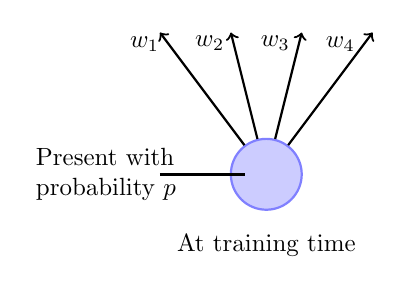
\begin{tikzpicture}[scale=.9, transform shape]
	\node[neuron,minimum width=1 cm] (A) at (2,0) {};
	\draw (0,0) node[text width=2.5cm] {Present with probability $p$};
	\draw[line width=1pt] (0.5,0) -- (1.7,0);
	\draw[thick,->] (A) -- (0.5,2) node[pos=.9,left] {$w_1$};
	\draw[thick,->] (A) -- (1.5,2) node[pos=.9,left] {$w_2$};
	\draw[thick,->] (A) -- (2.5,2) node[pos=.9,left] {$w_3$};
	\draw[thick,->] (A) -- (3.5,2) node[pos=.9,left] {$w_4$};
	\draw (2,-1) node[] {At training time};
\end{tikzpicture}
	\onslide<4->{
		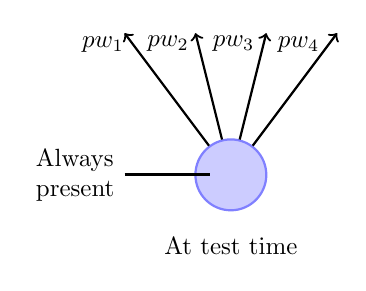
\begin{tikzpicture}[scale=.9, transform shape]
	\node[neuron,minimum width=1 cm] (A) at (2,0) {};
	\draw (0,0) node[text width=1.5cm] {Always present};
	\draw[line width=1pt] (0.5,0) -- (1.7,0);
	\draw[thick,->] (A) -- (0.5,2) node[pos=.9,left] {$pw_1$};
	\draw[thick,->] (A) -- (1.5,2) node[pos=.9,left] {$pw_2$};
	\draw[thick,->] (A) -- (2.5,2) node[pos=.9,left] {$pw_3$};
	\draw[thick,->] (A) -- (3.5,2) node[pos=.9,left] {$pw_4$};
	\draw (2,-1) node[] {At test time};
\end{tikzpicture}
	}
	\begin{itemize}
		\item<2-> What happens at test time?
		\item<3-> Impossible to aggregate the outputs of $2^n$ thinned networks
		\item<4-> Instead we use the full Neural Network and scale the output of each node by the fraction of times it was on during training
	\end{itemize}
						
\end{frame}
				
% \begin{frame}
% 	\hspace{1.8cm}
% 	\input{modules/Module11/tikz_images/backprop_network2.tex}
% 	\hspace{2cm}
% 	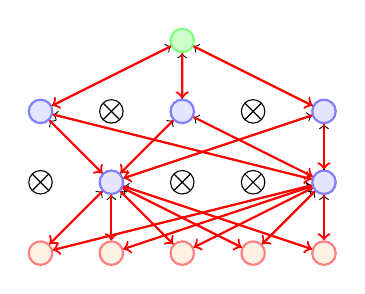
\begin{tikzpicture}[scale=.9, transform shape,cross/.style={path picture={ 
		\draw[black]
		(path picture bounding box.south east) -- (path picture bounding box.north west) (path picture bounding box.south west) -- (path picture bounding box.north east);
	}}]]
	\tikzstyle{mynode} = [draw,shape=circle]
	\tikzstyle{mycross} = [draw,shape=circle,cross]
	\node[input_neuron,mynode] (a0) at (0, 0) {};
	\node[input_neuron,mynode] (a1) at (1, 0) {};
	\node[input_neuron,mynode] (a2) at (2, 0) {};
	\node[input_neuron,mynode] (a3) at (3, 0) {};
	\node[input_neuron,mynode] (a4) at (4, 0) {};
	\node[mycross] (b0) at (0, 1) {};
	\node[hidden_neuron,mynode] (b1) at (1, 1) {};
	\node[mycross] (b2) at (2, 1) {};
	\node[mycross] (b3) at (3, 1) {};
	\node[hidden_neuron,mynode] (b4) at (4, 1) {};
	\node[hidden_neuron,mynode] (c0) at (0, 2) {};
	\node[mycross] (c1) at (1, 2) {};
	\node[hidden_neuron,mynode] (c2) at (2, 2) {};
	\node[mycross] (c3) at (3, 2) {};
	\node[hidden_neuron,mynode] (c4) at (4, 2) {};
	\node[output_neuron,mynode] (d2) at (2, 3) {};
	\foreach \from in {a0,a1,a2,a3,a4}
		\foreach \to in {b1,b4}
			\draw [->] (\from) -- (\to);
	\foreach \from in {b1,b4}
		\foreach \to in {c0,c2,c4}
			\draw [->] (\from) -- (\to);
	\foreach \from in {c0,c2,c4}
		\draw [->] (\from) -- (d2);
	\foreach \from in {c0,c2,c4}
		\draw<8-> [thick,red,->] (d2) -- (\from);
	\foreach \from in {b1,b4}
		\foreach \to in {c0,c2,c4}
			\draw<9-> [thick,red,->] (\to) -- (\from);
	\foreach \from in {a0,a1,a2,a3,a4}
		\foreach \to in {b1,b4}
			\draw<10-> [thick,red,->] (\to) -- (\from);
\end{tikzpicture}
				
% 	\begin{itemize}
% 		\justifying
% 		\item<2-> How do you do backpropagation in such a noisy network which changes for each training instance (or batch)
% 		\item<3-> Simple: we only backpropagate over the paths which are active and only update those weights which are active in the current thinned network
% 	\end{itemize}
% \end{frame}
					
\begin{frame}
	\begin{columns}									
		\column{0.5\textwidth}
		\begin{overlayarea}{\textwidth}{\textheight}
			\vspace{1cm}
			\hspace{1cm}
			\input{modules/Module11/tikz_images/f_backprop_dropout_network2.tex}
		\end{overlayarea}									
		\column{0.5\textwidth}
		\begin{overlayarea}{\textwidth}{\textheight}
			\begin{itemize}
				\justifying
				\item Dropout essentially applies a masking noise to the hidden units
				\item<2-> Prevents hidden units from co-adapting
				\item<3-> Essentially a hidden unit cannot rely too much on other units as they may get dropped out any time
				\item<4-> Each hidden unit has to learn to be more robust to these random dropouts
			\end{itemize}
		\end{overlayarea}
	\end{columns}
\end{frame}
						
\begin{frame}
	\begin{columns}
										
		\column{0.5\textwidth}
		\begin{overlayarea}{\textwidth}{\textheight}
			\vspace{1cm}
			\hspace{1cm}
			\input{modules/Module11/tikz_images/h_network2.tex}
		\end{overlayarea}
										
		\column{0.5\textwidth}
		\begin{overlayarea}{\textwidth}{\textheight}
			\begin{itemize}\justifying
				\item<2-> Here is an example of how dropout helps in ensuring redundancy and robustness
				\item<3-> Suppose $h_i$ learns to detect a face by firing on detecting a nose
				\item<4-> Dropping $h_i$ then corresponds to erasing the information that  a nose exists
				\item<5-> The model should then learn another $h_i$ which redundantly encodes the presence of a nose
				\item<6-> Or the model should learn to detect the face using other features
			\end{itemize}
		\end{overlayarea}
	\end{columns}
\end{frame}

\begin{frame}
	\vspace{4em}
	\begin{overlayarea}{\textwidth}{\textheight}
		\begin{block}{Recap}
			\begin{itemize}
				\item $l_2$ regularization
				\item Dataset augmentation
				\item Parameter Sharing and tying
				\item Adding Noise to the inputs
				\item Adding Noise to the outputs 
				\item Early stopping
				\item Ensemble methods
				\item Dropout
			\end{itemize}
		\end{block}
	\end{overlayarea}
\end{frame}
				
				
		%%%%%%%%%%%%The End%%%%%%%%%%%%%%%%%%%%%%%%%%%%%%%%%%%5555
				
				
